\section{Zadanie 2}

Drugie zadanie polegało na wyznaczeniu cech holistycznie dla różnej liczby estymowanych komponentów głównych(J = 4, 10, 20, 30). Obrazy oryginalne i redukowane zostały pogrupowane metodą k-średnich. Badania zostały przeprowadzone dla liczby grup od 2 do 5 w środowisku Matlab oraz zmierzono czas i porównano dokładność grupowania. Następnie dokonano klasyfikacji obrazów w przestrzeni oryginalnej i zredukowanej przy pomocy klasyfikatora K-NN. Na koniec efekty klasyfikacji zostały porównane z efektami grupowania.



\begin{figure}[H]
	\centering
	\hspace*{-1.2in}
	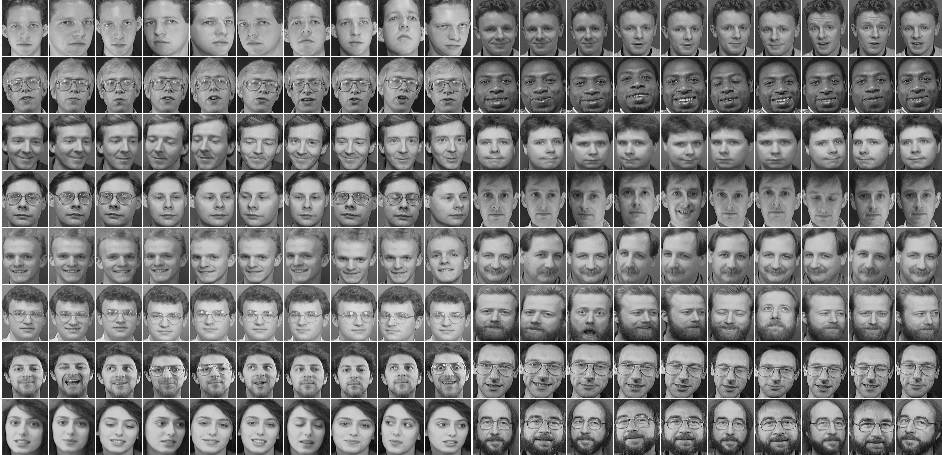
\includegraphics[scale = 0.6]{faces.jpg}
	\caption{Zdjęcia twarzy, z których wybrano kilka grup do klasyfikacji}  
	\label{rys:faces} 
\end{figure}

\subsection{Implementacja główna}

Na poniższym listingu została przedstawiona główna pętla programu. Podczas jej działania zostają wykonane następujące operacje:
\begin{itemize}
	\item Wczytanie wybranej ilości folderów ze zdjęciami,
	\item Utworzenie wzorcowego wektora, zawierającego klasy kolejnych obrazów (klasa - numer osoby, której zrobiono zdjęcie), 
	\item Dla każdej z wskazanych wartości estymowanych komponentów głównych (J) zostaje przeprowadzone zredukowanie wymiarów za pomocą funkcji \textit{myPCA},
	\item Zdjęcia oryginalne oraz zredukowane zostają poddane grupowaniu i klasyfikacji,
	\item Zapis skuteczności i czasu działania algorytmów do plików.
\end{itemize}

Pętla ta jest wykonywana dla różnej liczby klas (grup) zdjęć, w zależności od zmiennej \textit{classes\_count}.

\vspace{5mm}

\begin{lstlisting}[linewidth=16.0cm][caption={[Skrypt main, wykonujący kod główny]}]
classes_count = 5;
% Wczytywanie zdjec dla wybranej liczy klas
images_arrays = getAllImages(classes_count);
	
J = [4, 10, 20, 30];
iterations = 10;
	
% Wektor zawierajacy klasy kolejnych obrazow
images_classes = [];
for i = 1:classes_count
	images_classes =[images_classes; ones(10,1).*i];
end
	
% Petla glowna
for j_val = 1:4
	grouping_results = zeros([iterations 4]);
	classification_results = zeros([iterations 4]);
	
	for i = 1 : iterations
		% Redukcja wymiarow
		[V, pca_images_arrays, D] = myPCA(images_arrays', J(j_val));
		
		% Grupowanie za pomoca k-srednich
		g_result = getGroupingResults(
		images_arrays, pca_images_arrays, classes_count, 
		images_classes);
		grouping_results(i,:) = g_result;
		
		% Klasyfikacja z uzyciem k-NN
		c_result = getClassificationResults(
		images_arrays, pca_images_arrays, classes_count, 
		images_classes);
		classification_results(i,:) = c_result;
	end
	
	% Zapis wynikow do plikow
	(...)
end
\end{lstlisting}

\vspace{5mm}

W celu redukcji wymiarów za pomocą algorytmu PCA, została zaimplementowana funkcja \textit{myPCA}, którą przedstawiono poniżej.

\vspace{5mm}

\begin{lstlisting}[linewidth=16.0cm]
function [V, newX, D] = myPCA(X, J)
	X = bsxfun(@minus, X, mean(X,2));
	C = (X*X')./(size(X,2)-1);
	
	[V, D] = eigs(C,J);
	[D, order] = sort(diag(D), 'descend');
	V = V(:, order);
	newX = V'*X;
end
\end{lstlisting}


\subsection{Implementacja grupowania}

Pierwszym krokiem do rozwiązania zadania było pogrupowanie zdjęć z użyciem algorytmu k-średnich. W tym celu powstała funkcja \textit{getGroupingResults}. 

\vspace{5mm} 

\begin{lstlisting}[linewidth=16.0cm]
function result = getGroupingResults(images_arrays, pca_images_arrays, 
	clusters, images_classes)
	
	% Uruchomienie grupowania k-srednich,
	% Zapis wynikow i czasu trwania
	tic;
	groups = kmeans(images_arrays, clusters);
	default_time = toc;
	tic;
	groups_pca = kmeans(pca_images_arrays', clusters);
	pca_time = toc;
	
	% Obliczenie skutecznosci grupowania i jej normalizacja
	default_acc = AccMeasure(images_classes, groups)/100.0;
	pca_acc = AccMeasure(images_classes, groups_pca)/100.0;
	
	result = [default_acc, pca_acc, default_time, pca_time];
end
\end{lstlisting}

\vspace{5mm} 

Jak można zauważyć na powyższym listingu, funkcja przyjmuje 4 argumenty:
\begin{itemize}
	\item \textit{images\_arrays} - oryginalne macierze zdjęć,
	\item \textit{pca\_images\_arrays} - macierze zdjęc po redukcji wymiarów,
	\item \textit{clusters} - ilość klastrów (grup) zdjęć,
	\item \textit{images\_classes} - wzorzec klas dla kolejnych zdjęć.
\end{itemize}
Podczas wykonywania funkcji mierzony jest czas grupowania, a następnie, za pomocą funkcji \textit{AccMeasure}, także jej skuteczność. Numery klas przyporządkowanych kolejnym obrazom w wyniku grupowania k-średnich nie zawsze są tożsame z tymi, które zostały podane jako wzorcowe. Jednak \textit{AccMeasure} radzi sobie z przyporządkowaniem klas założonych klasom otrzymanym ze skutecznością ponad 80\%. Można to sprawdzić, uruchamiając ją w ten sposób, by zwracała trzy wartości - jedna z nich przedstawia właśnie tą skuteczność. Wyniki otrzymane za pomocą tej funkcji należy znormalizować tak, by największa możliwa ich wartość była równa 1. Wtedy można łatwo porównać je z wynikami klasyfikacji.\\
Ostatecznie otrzymujemy skuteczność i czas grupowań zdjęć oryginalnych i tych po redukcji wymiarów.

\subsection{Implementacja klasyfikacji}

Kolejnym elementem implementacji jest klasyfikacja obrazów za pomocą algorytmu k najbliższych sąsiadów. W tym celu została stworzona funkcja \textit{getClassificationResults}. Przyjmuje ona te same argumenty, co funkcja używana przy grupowaniu, jednak dla lepszego zrozumienia działania kodu zmiennej \textit{clusters} z poprzedniego listingu odpowiada \textit{classes\_count} z obecnego.

\vspace{5mm} 

\begin{lstlisting}[linewidth=16.0cm]
function result = getClassificationResults(images_arrays, pca_images_arrays,
 classes_count, images_classes)

	% Uruchomienie klasyfikacji k-NN,
	% Zapis wynikow i czasu trwania
	tic;
	model = fitcknn(images_arrays, images_classes);
	cv_model = crossval(model,'KFold',classes_count);
	default_time = toc;
	tic;
	model_pca = fitcknn(pca_images_arrays', images_classes);
	cv_model_pca = crossval(model_pca,'KFold',classes_count);
	pca_time = toc;
	
	% Obliczenie skutecznosci grupowania
	cv_model_loss = kfoldLoss(cv_model);
	default_acc = 1 - cv_model_loss;
	cv_model_pca_loss = kfoldLoss(cv_model_pca);
	pca_acc = 1 - cv_model_pca_loss;
	
	result = [default_acc, pca_acc, default_time, pca_time];
\end{lstlisting}

\vspace{5mm} 

Najpierw, na podstawie macierzy obrazów i wzorca ich klas, za pomocą algorytmu k-NN, tworzony jest model klasyfikatora. Następnie, z wykorzystanie fukcji \textit{crossval}, przeprowadzona zostaje kroswalidacja, czyli analiza modelu, polegająca na wybraniu przez algorytm różnych elementów zbioru jako zestaw uczący, a jednego jako testowy. Taki sprawdzian zostaje przeprowadzony dla wielu kombinacji elementów w grupach. Ostatnim krokiem jest sprawdzenie błędu modelu za pomocą funkcji \textit{kfoldLoss}. Odejmując wynik od liczby 1 otrzymujemy skuteczność klasyfikacji w modelu. 


\subsection{Wyniki}

\subsubsection{Grupowanie}

\begin{figure}[H]
	\centering
	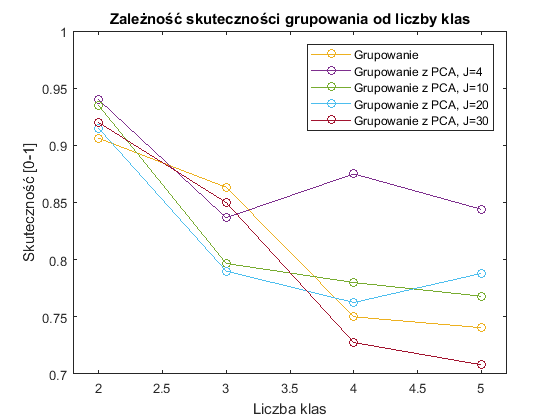
\includegraphics{img/acc_from_classes_group.png}
	\caption{Skuteczność grupowania dla wymiarów pełnych i zredukowanych}  
	\label{rys:acc_from_classes_group} 
\end{figure}

Na wykresie można zauważyć, że zwkle skuteczność grupowania spada wraz ze wzrostem ilości klas. Najgorzej w tym podsumowaniu wypadają zdjęcia po zdredukowaniu wymiarów do J=30, natomiast w pozytywny sposób wyróżnia się PCA z J=4 wymiarami.

\begin{figure}[H]
	\centering
	\hspace*{-0.8in}
	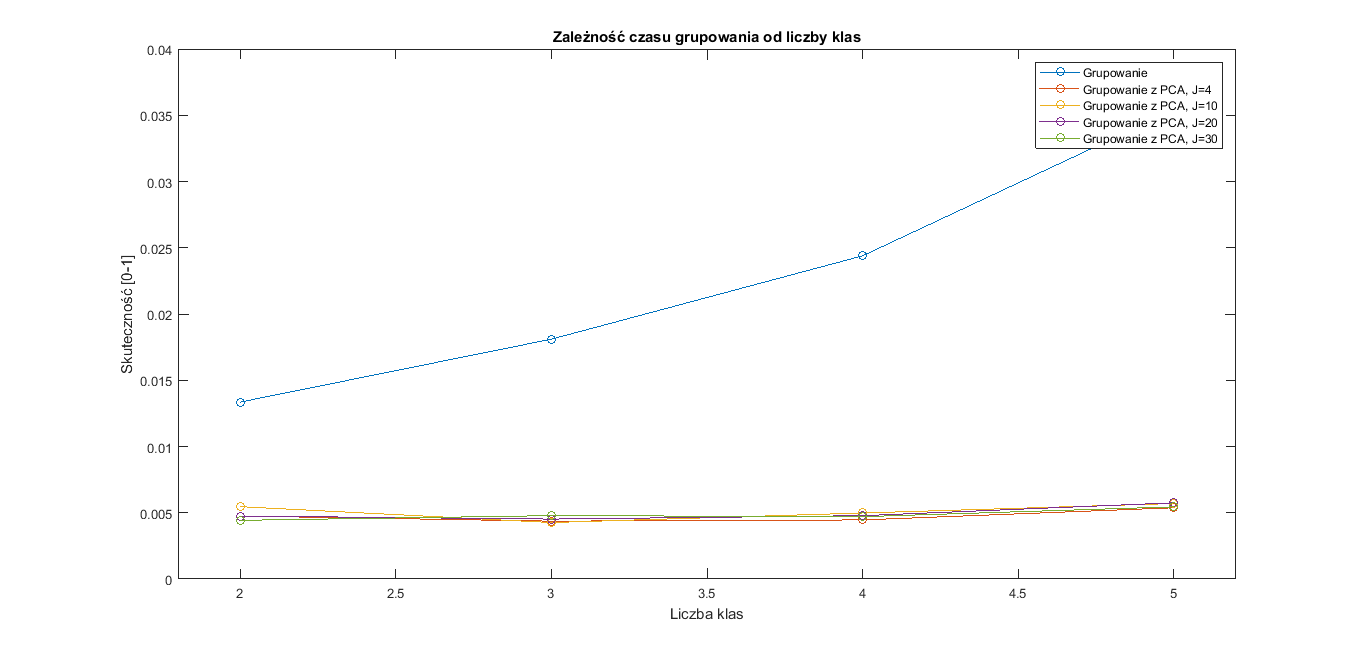
\includegraphics[scale = 0.5]{img/time_from_classes_group.png}
	\caption{Czas grupowania dla wymiarów pełnych i zredukowanych}  
	\label{rys:time_from_classes_group} 
\end{figure}

Na wykresie jasno widać, że redukcja wymiarów w każdym przypadku znacząco wpłynęła na redukcję czasu grupowania.

\subsubsection{Porównanie klasyfikacji i grupowania}

\begin{figure}[H]
	\centering
	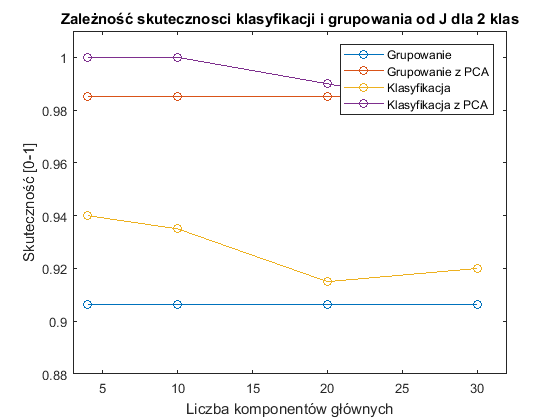
\includegraphics{img/acc_from_J_2classes.png}
	\caption{Skuteczność grupowania i klasyfikacji dla 2 klas}  
	\label{rys:acc_from_J_2classes} 
\end{figure}

\begin{figure}[H]
	\centering
	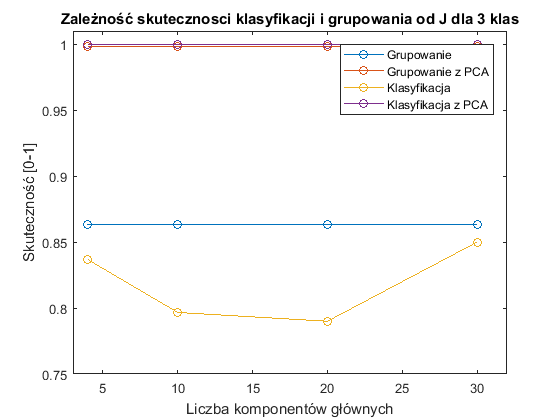
\includegraphics{img/acc_from_J_3classes.png}
	\caption{Skuteczność grupowania i klasyfikacji dla 3 klas}  
	\label{rys:acc_from_J_3classes} 
\end{figure}

\begin{figure}[H]
	\centering
	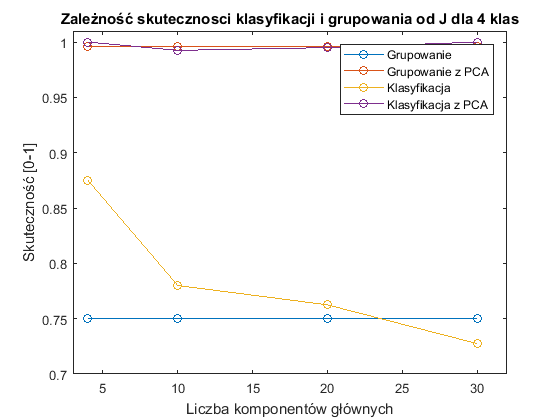
\includegraphics{img/acc_from_J_4classes.png}
	\caption{Skuteczność grupowania i klasyfikacji dla 4 klas}  
	\label{rys:acc_from_J_42classes} 
\end{figure}

\begin{figure}[H]
	\centering
	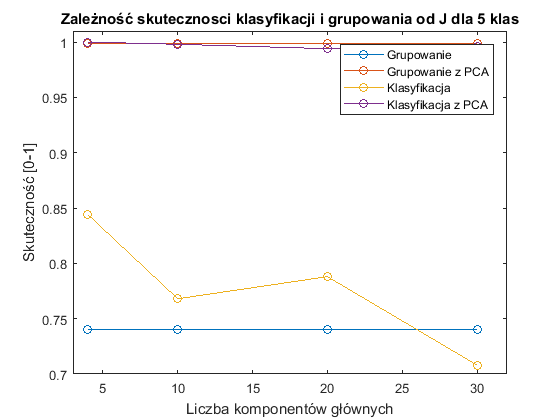
\includegraphics{img/acc_from_J_5classes.png}
	\caption{Skuteczność grupowania i klasyfikacji dla 5 klas}  
	\label{rys:acc_from_J_5classes} 
\end{figure}

\begin{figure}[H]
	\centering
	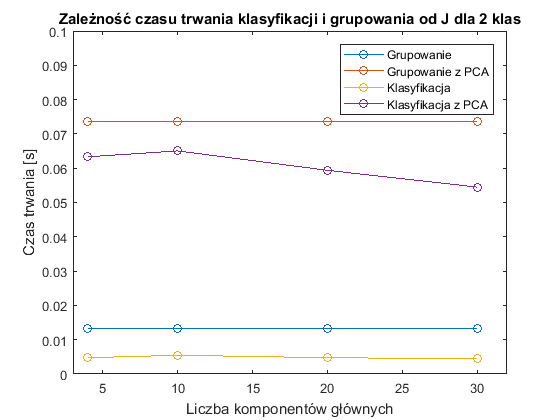
\includegraphics{img/time_from_J_2classes.png}
	\caption{Czas grupowania i klasyfikacji dla 2 klas}  
	\label{rys:time_from_J_2classes} 
\end{figure}

\begin{figure}[H]
	\centering
	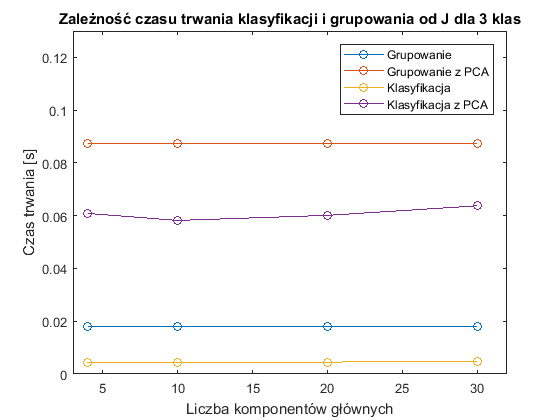
\includegraphics{img/time_from_J_3classes.png}
	\caption{Czas grupowania i klasyfikacji dla 3 klas}  
	\label{rys:time_from_J_3classes} 
\end{figure}

\begin{figure}[H]
	\centering
	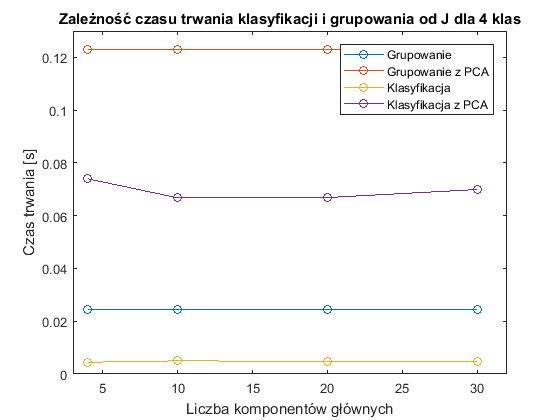
\includegraphics{img/time_from_J_4classes.png}
	\caption{Czas grupowania i klasyfikacji dla 4 klas}  
	\label{rys:time_from_J_42classes} 
\end{figure}

\begin{figure}[H]
	\centering
	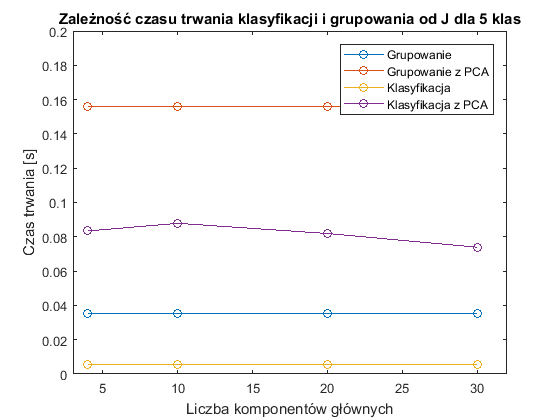
\includegraphics{img/time_from_J_5classes.png}
	\caption{Czas grupowania i klasyfikacji dla 5 klas}  
	\label{rys:time_from_J_5classes} 
\end{figure}


Zarówno w przypadku grupowania, jak i klasyfikacji, zastosowanie PCA korzystnie wpływa na skuteczność działania algorytmów. Jeśli chodzi o czas wykonywania programu, jest on dłuższy przy użyciu obrazów zredukowanych przez algorytm PCA.